%%%%%%%%%%%%%%%%%%%%%%%%%%%%%%%%%%%%%%%%%%%%%%%%%%%
\begin{frame}
  \begin{center}
    {\Large Neural Network from scratch}
    
    (Ref: Andrew Trask, Milo Spencer-Harper)
  \end{center}
\end{frame}


%%%%%%%%%%%%%%%%%%%%%%%%%%%%%%%%%%%%%%%%%%%%%%%%%%%
\begin{frame}[fragile] \frametitle{Simple Problem}
\begin{center}
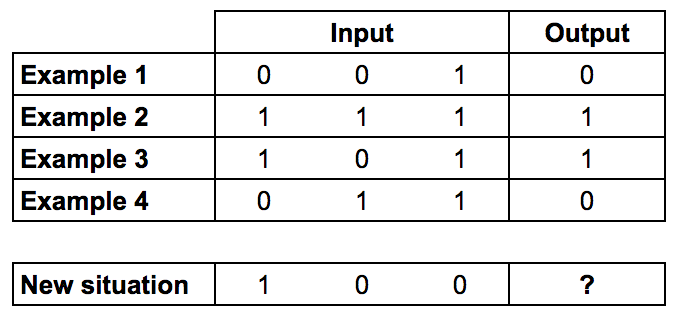
\includegraphics[width=0.8\linewidth,keepaspectratio]{ttn1}
\end{center}
\end{frame}

%%%%%%%%%%%%%%%%%%%%%%%%%%%%%%%%%%%%%%%%%%%%%%%%%%%
\begin{frame}[fragile] \frametitle{A Tiny Toy Network}
\begin{center}
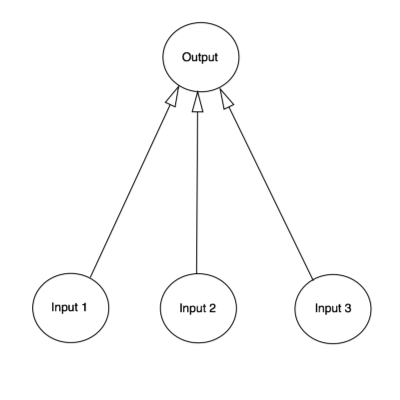
\includegraphics[width=0.6\linewidth,keepaspectratio]{ttn2}
\end{center}
\end{frame}


%%%%%%%%%%%%%%%%%%%%%%%%%%%%%%%%%%%%%%%%%%%%%%%%%%%
\begin{frame}[fragile] \frametitle{Training process}
\begin{itemize}
\item We will give each input a weight, which can be a positive or negative number. 
\item An input with a large positive weight or a large negative weight, will have a strong effect on the neuron's output. 
\item Before we start, we set each weight to a random number. 
\item Then we begin the training process.

\end{itemize}
\end{frame}


%%%%%%%%%%%%%%%%%%%%%%%%%%%%%%%%%%%%%%%%%%%%%%%%%%%
\begin{frame}[fragile] \frametitle{Training process}
\begin{itemize}
\item Take the inputs from a training set example, adjust them by the weights, and pass them through a special formula to calculate the neuron's output.
\item Calculate the error, which is the difference between the neuron's output and the desired output in the training set example.
\item Depending on the direction of the error, adjust the weights slightly.
\item Repeat this process 10, 000 times.
\end{itemize}
\end{frame}


%%%%%%%%%%%%%%%%%%%%%%%%%%%%%%%%%%%%%%%%%%%%%%%%%%%
\begin{frame}[fragile] \frametitle{Training process}
\begin{itemize}
\item Eventually the weights of the neuron will reach an optimum for the training set.
\item This process is called back propagation.
\end{itemize}
\begin{center}
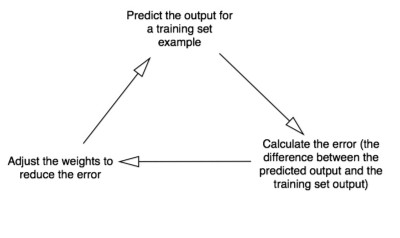
\includegraphics[width=\linewidth,keepaspectratio]{ttn3}
\end{center}
\end{frame}


%%%%%%%%%%%%%%%%%%%%%%%%%%%%%%%%%%%%%%%%%%%%%%%%%%%
\begin{frame}[fragile] \frametitle{Formula for calculating the neuron's output}
\begin{itemize}
\item First we take the weighted sum of the neuron's inputs:
\begin{center}
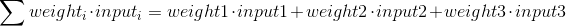
\includegraphics[width=\linewidth,keepaspectratio]{ttn4}
\end{center}
\item Next we normalize this, so the result is between 0 and 1 usinng Sigmoid function
\begin{center}
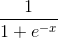
\includegraphics[width=0.1\linewidth,keepaspectratio]{ttn5}
\end{center}
\end{itemize}
\end{frame}


%%%%%%%%%%%%%%%%%%%%%%%%%%%%%%%%%%%%%%%%%%%%%%%%%%%
\begin{frame}[fragile] \frametitle{Formula for calculating the neuron's output}
\begin{itemize}
\item So by substituting the first equation into the second, the final formula for the output of the neuron is:
\begin{center}
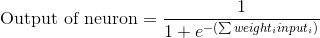
\includegraphics[width=0.6\linewidth,keepaspectratio]{ttn6}
\end{center}
\item If plotted on a graph, the Sigmoid function draws an S shaped curve.
\begin{center}
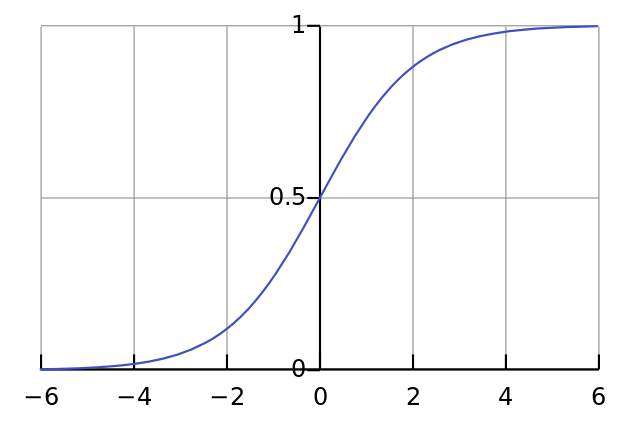
\includegraphics[width=0.6\linewidth,keepaspectratio]{ttn7}
\end{center}
\end{itemize}
\end{frame}

%%%%%%%%%%%%%%%%%%%%%%%%%%%%%%%%%%%%%%%%%%%%%%%%%%%
\begin{frame}[fragile] \frametitle{Formula for adjusting the weights}
\begin{itemize}
\item During the training cycle, we adjust the weights useing the ``Error Weighted Derivative'' formula:
\begin{center}
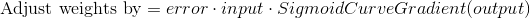
\includegraphics[width=\linewidth,keepaspectratio]{ttn8}
\end{center}
\item First we want to make the adjustment proportional to the size of the error.
\item Secondly, we multiply by the input, which is either a 0 or a 1. If the input is 0, the weight isn't adjusted. 
\item Finally, we multiply by the gradient of the Sigmoid curve
\end{itemize}
\end{frame}

%%%%%%%%%%%%%%%%%%%%%%%%%%%%%%%%%%%%%%%%%%%%%%%%%%
\begin{frame}[fragile] \frametitle{Formula for adjusting the weights}
\begin{itemize}
\item     We used the Sigmoid curve to calculate the output of the neuron.
\item     If the output is a large positive or negative number, it signifies the neuron was quite confident one way or another.
\item     We can see that at large numbers, the Sigmoid curve has a shallow gradient.
\item      If the neuron is confident that the existing weight is correct, it doesn't want to adjust it very much. 
\item Multiplying by the Sigmoid curve gradient achieves this.
\end{itemize}
\end{frame}

%%%%%%%%%%%%%%%%%%%%%%%%%%%%%%%%%%%%%%%%%%%%%%%%%%%
\begin{frame}[fragile] \frametitle{Formula for calculating the neuron's output}
\begin{itemize}
\item The gradient of the Sigmoid curve, can be found by taking the derivative:
\begin{center}
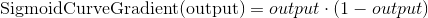
\includegraphics[width=0.8\linewidth,keepaspectratio]{ttn9}
\end{center}
\item So by substituting the second equation into the first equation, the final formula for adjusting the weights is:
\begin{center}
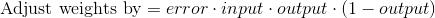
\includegraphics[width=0.8\linewidth,keepaspectratio]{ttn10}
\end{center}
\item There are alternative formulae, which would allow the neuron to learn more quickly, but this one has the advantage of being fairly simple.
\end{itemize}
\end{frame}


%%%%%%%%%%%%%%%%%%%%%%%%%%%%%%%%%%%%%%%%%%%%%%%%%%%
\begin{frame}[fragile] \frametitle{Python Implementation}
\begin{itemize}
\item Use the numpy array() method to represent the training set 
\begin{lstlisting}
training_set_inputs = array([[0, 0, 1], [1, 1, 1], [1, 0, 1], [0, 1, 1]])
training_set_outputs = array([[0, 1, 1, 0]]).T
\end{lstlisting}
\item The ‘.T’ function, transposes the matrix from horizontal to vertical. So the computer is storing the numbers like this.
\begin{center}
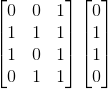
\includegraphics[width=0.2\linewidth,keepaspectratio]{ttn11}
\end{center}
\end{itemize}
\end{frame}

%%%%%%%%%%%%%%%%%%%%%%%%%%%%%%%%%%%%%%%%%%%%%%%%%%%
\begin{frame}[fragile] \frametitle{Inputs and Outputs}

\begin{lstlisting}
# input dataset
X = np.array([  [0,0,1],
                [0,1,1],
                [1,0,1],
                [1,1,1] ])
    
# output dataset            
y = np.array([[0,0,1,1]]).T
\end{lstlisting}
\end{frame}


%%%%%%%%%%%%%%%%%%%%%%%%%%%%%%%%%%%%%%%%%%%%%%%%%%%
\begin{frame}[fragile] \frametitle{Inputs and Outputs}

\begin{lstlisting}
import numpy as np

# input dataset
X = np.array([  [0,0,1],
                [0,1,1],
                [1,0,1],
                [1,1,1] ])
    
# output dataset            
y = np.array([[0,0,1,1]]).T
\end{lstlisting}
\end{frame}


%%%%%%%%%%%%%%%%%%%%%%%%%%%%%%%%%%%%%%%%%%%%%%%%%%%
\begin{frame}[fragile] \frametitle{Sigmoid}

\begin{lstlisting}
# sigmoid function
def nonlin(x,deriv=False):
    if(deriv==True):
        return x*(1-x)
    return 1/(1+np.exp(-x))
\end{lstlisting}
\end{frame}

%%%%%%%%%%%%%%%%%%%%%%%%%%%%%%%%%%%%%%%%%%%%%%%%%%%
\begin{frame}[fragile] \frametitle{Initialization}

\begin{lstlisting}
# seed random numbers to make calculation
# deterministic (just a good practice)
np.random.seed(1)

# initialize weights randomly with mean 0
syn0 = 2*np.random.random((3,1)) - 1 # First layer of weights, Synapse 0, connecting l0 to l1.
\end{lstlisting}
\end{frame}


%%%%%%%%%%%%%%%%%%%%%%%%%%%%%%%%%%%%%%%%%%%%%%%%%%%
\begin{frame}[fragile] \frametitle{Core}

\begin{lstlisting}
for iter in xrange(10000):

    l0 = X #First Layer of the Network, specified by the input data
    l1 = nonlin(np.dot(l0,syn0)) #Second Layer of the Network, otherwise known as the hidden layer

    # how much did we miss?
    l1_error = y - l1

    # multiply how much we missed by the 
    # slope of the sigmoid at the values in l1
    l1_delta = l1_error * nonlin(l1,True) 

    # update weights
    syn0 += np.dot(l0.T,l1_delta)

print("Output After Training: {}".format(l1))
\end{lstlisting}
\end{frame}

%%%%%%%%%%%%%%%%%%%%%%%%%%%%%%%%%%%%%%%%%%%%%%%%%%%
\begin{frame}[fragile] \frametitle{Core}
Note:
\begin{itemize}
\item $*$: Elementwise multiplication, so two vectors of equal size are multiplying corresponding values 1-to-1 to generate a final vector of identical size.
\item $-$:  Elementwise subtraction, so two vectors of equal size are subtracting corresponding values 1-to-1 to generate a final vector of identical size.
\item $x.dot(y)$ : If x and y are vectors, this is a dot product. If both are matrices, it's a matrix-matrix multiplication. If only one is a matrix, then it's vector matrix multiplication.
\end{itemize}
\end{frame}


%%%%%%%%%%%%%%%%%%%%%%%%%%%%%%%%%%%%%%%%%%%%%%%%%%%
\begin{frame}[fragile] \frametitle{Explanation}

\begin{itemize}
\item Our first layer, l0, is simply our data.
\item X contains 4 training examples (rows). We're going to process all of them at the same time in this implementation. 
\item This is known as ``full batch'' training. 
\end{itemize}
\end{frame}

%%%%%%%%%%%%%%%%%%%%%%%%%%%%%%%%%%%%%%%%%%%%%%%%%%%
\begin{frame}[fragile] \frametitle{Explanation}

\begin{itemize}
\item \lstinline| l1 = nonlin(np.dot(l0,syn0))| is the prediction step.
\item Basically, we first let the network "try" to predict the output given the input. 
\item We will then study how it performs so that we can adjust it to do a bit better for each iteration. 
\item This line contains 2 steps. The first matrix multiplies l0 by syn0. The second passes our output through the sigmoid function.
\item Since we loaded in 4 training examples, we ended up with 4 guesses for the correct answer, a (4 x 1) matrix.
\end{itemize}
\end{frame}


%%%%%%%%%%%%%%%%%%%%%%%%%%%%%%%%%%%%%%%%%%%%%%%%%%%
\begin{frame}[fragile] \frametitle{Explanation}

\begin{itemize}
\item \lstinline|l1_error = y - l1| 
\item Given that l1 had a ``guess'' for each input. 
\item We can now compare how well it did by subtracting the true answer (y) from the guess (l1).
\item  l1\_error is just a vector of positive and negative numbers reflecting how much the network missed. 
\end{itemize}
\end{frame}

%%%%%%%%%%%%%%%%%%%%%%%%%%%%%%%%%%%%%%%%%%%%%%%%%%%
\begin{frame}[fragile] \frametitle{Explanation}

\begin{itemize}
\item \lstinline|l1_delta = l1_error * nonlin(l1,True)|
\item If l1 represents these three points on the sigmoid curve, then \lstinline|nonlin(l1,True)| generates the slopes of the lines below.
\begin{center}
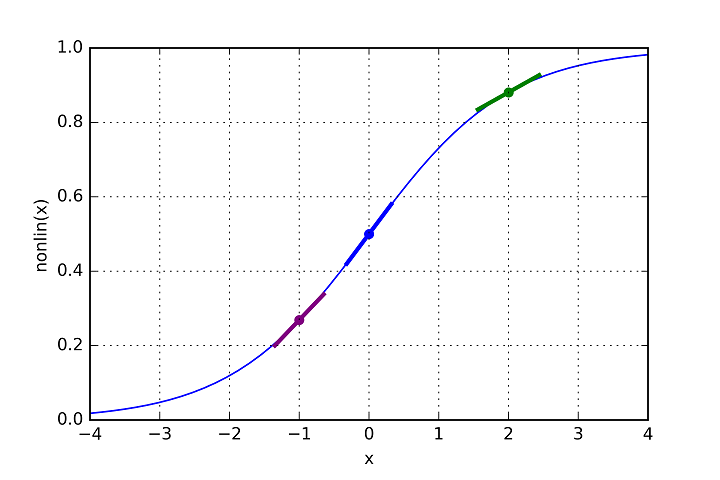
\includegraphics[width=0.8\linewidth,keepaspectratio]{ttn12}
\end{center}
\end{itemize}
\end{frame}

%%%%%%%%%%%%%%%%%%%%%%%%%%%%%%%%%%%%%%%%%%%%%%%%%%%
\begin{frame}[fragile] \frametitle{Explanation}

\begin{itemize}
\item Notice that very high values such as x=2.0 (green dot) and very low values such as x=-1.0 (purple dot) have rather shallow slopes.
\item The highest slope you can have is at x=0 (blue dot). 
\item This plays an important role. 
\item Also notice that all derivatives are between 0 and 1. 
\end{itemize}
\end{frame}

%%%%%%%%%%%%%%%%%%%%%%%%%%%%%%%%%%%%%%%%%%%%%%%%%%%
\begin{frame}[fragile] \frametitle{Explanation}

\begin{itemize}
\item \lstinline|l1_delta = l1_error * nonlin(l1,True)|
\item  l1\_error is a (4,1) matrix.
\item nonlin(l1,True) returns a (4,1) matrix. 
\item $*$ returns a (4,1) matrix l1\_delta with the multiplied values. 
\end{itemize}
\end{frame}

%%%%%%%%%%%%%%%%%%%%%%%%%%%%%%%%%%%%%%%%%%%%%%%%%%%
\begin{frame}[fragile] \frametitle{Explanation}

\begin{itemize}
\item When we multiply the ``slopes'' by the error, we are reducing the error of high confidence predictions. 
\item If the slope was really shallow (close to 0), then the network either had a very high value, or a very low value. 
\item This means that the network was quite confident one way or the other.
\end{itemize}
\end{frame}

%%%%%%%%%%%%%%%%%%%%%%%%%%%%%%%%%%%%%%%%%%%%%%%%%%%
\begin{frame}[fragile] \frametitle{Explanation}

\begin{itemize}
\item However, if the network guessed something close to (x=0, y=0.5) then it isn't very confident. 
\item We update these ``wishy-washy'' predictions most heavily, and we tend to leave the confident ones alone by multiplying them by a number close to 0. 
\end{itemize}
\end{frame}

%%%%%%%%%%%%%%%%%%%%%%%%%%%%%%%%%%%%%%%%%%%%%%%%%%%
\begin{frame}[fragile] \frametitle{Explanation}
We are now ready to update our network! Let's take a look at a single training example. 
\begin{center}
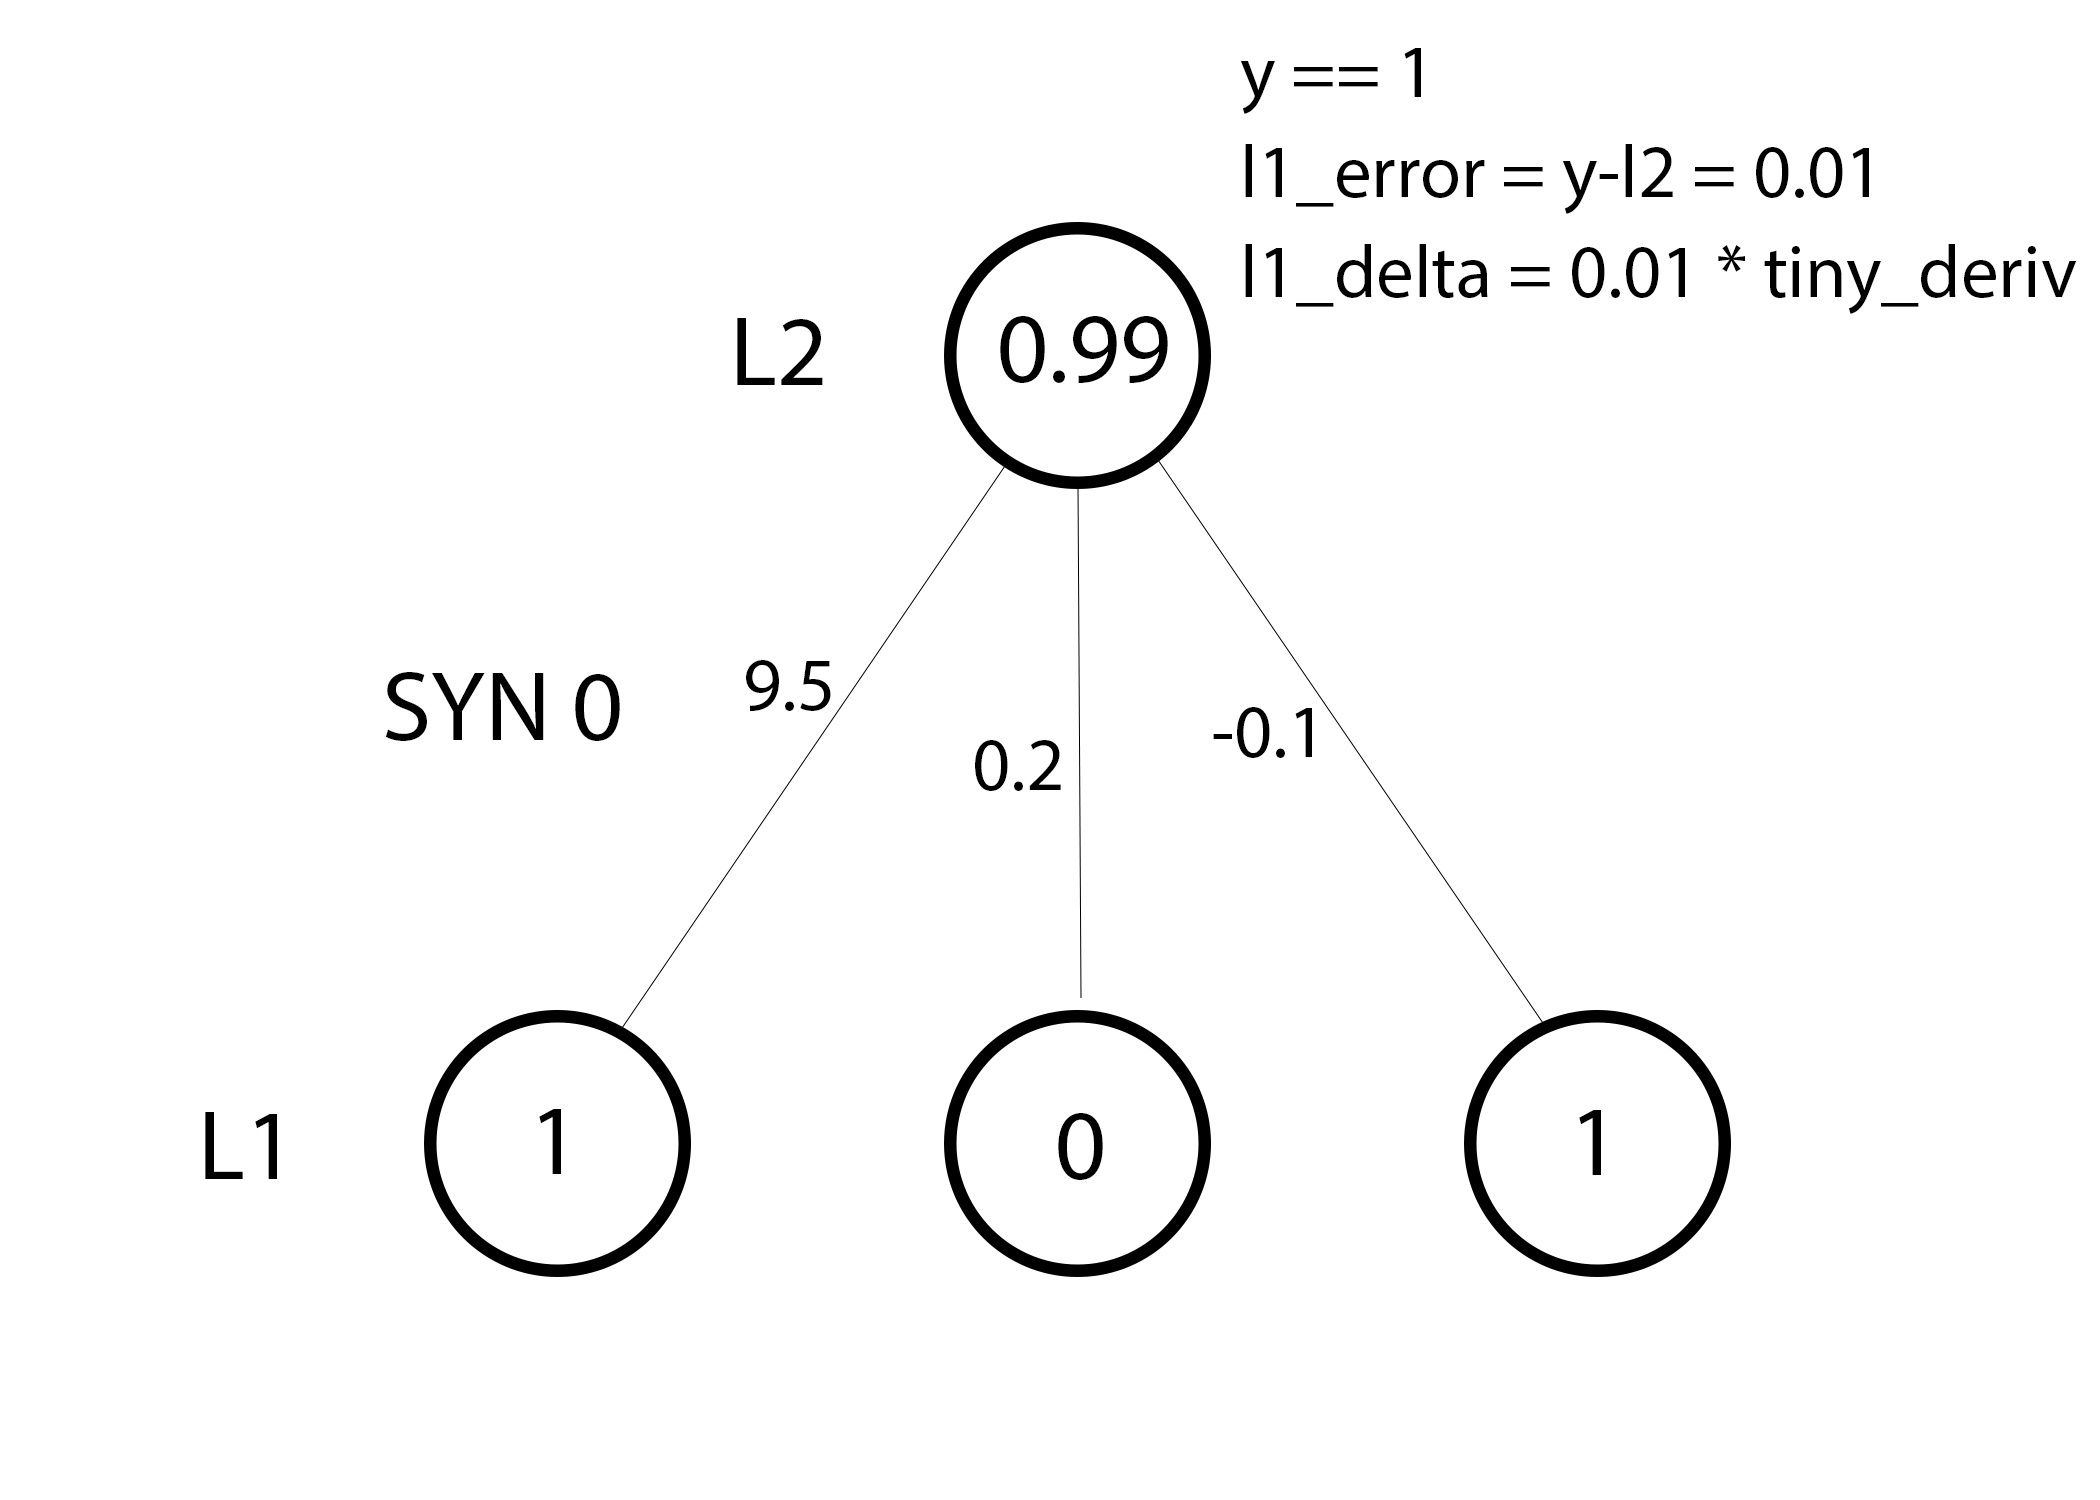
\includegraphics[width=0.8\linewidth,keepaspectratio]{ttn13}
\end{center}
\end{frame}

%%%%%%%%%%%%%%%%%%%%%%%%%%%%%%%%%%%%%%%%%%%%%%%%%%%
\begin{frame}[fragile] \frametitle{Explanation}
Let's update the far left weight (9.5): weight\_update = input\_value * l1\_delta
\begin{itemize}
\item For the far left weight, this would multiply 1.0 * the l1\_delta. Presumably, this would increment 9.5 ever so slightly. 
\item Why only a small amount? Well, the prediction was already very confident, and the prediction was largely correct.
\item  A small error and a small slope means a VERY small update. 
\end{itemize}
\end{frame}


%%%%%%%%%%%%%%%%%%%%%%%%%%%%%%%%%%%%%%%%%%%%%%%%%%%
\begin{frame}[fragile] \frametitle{Explanation}
Consider all the weights. It would ever so slightly increase all three. 
\begin{center}
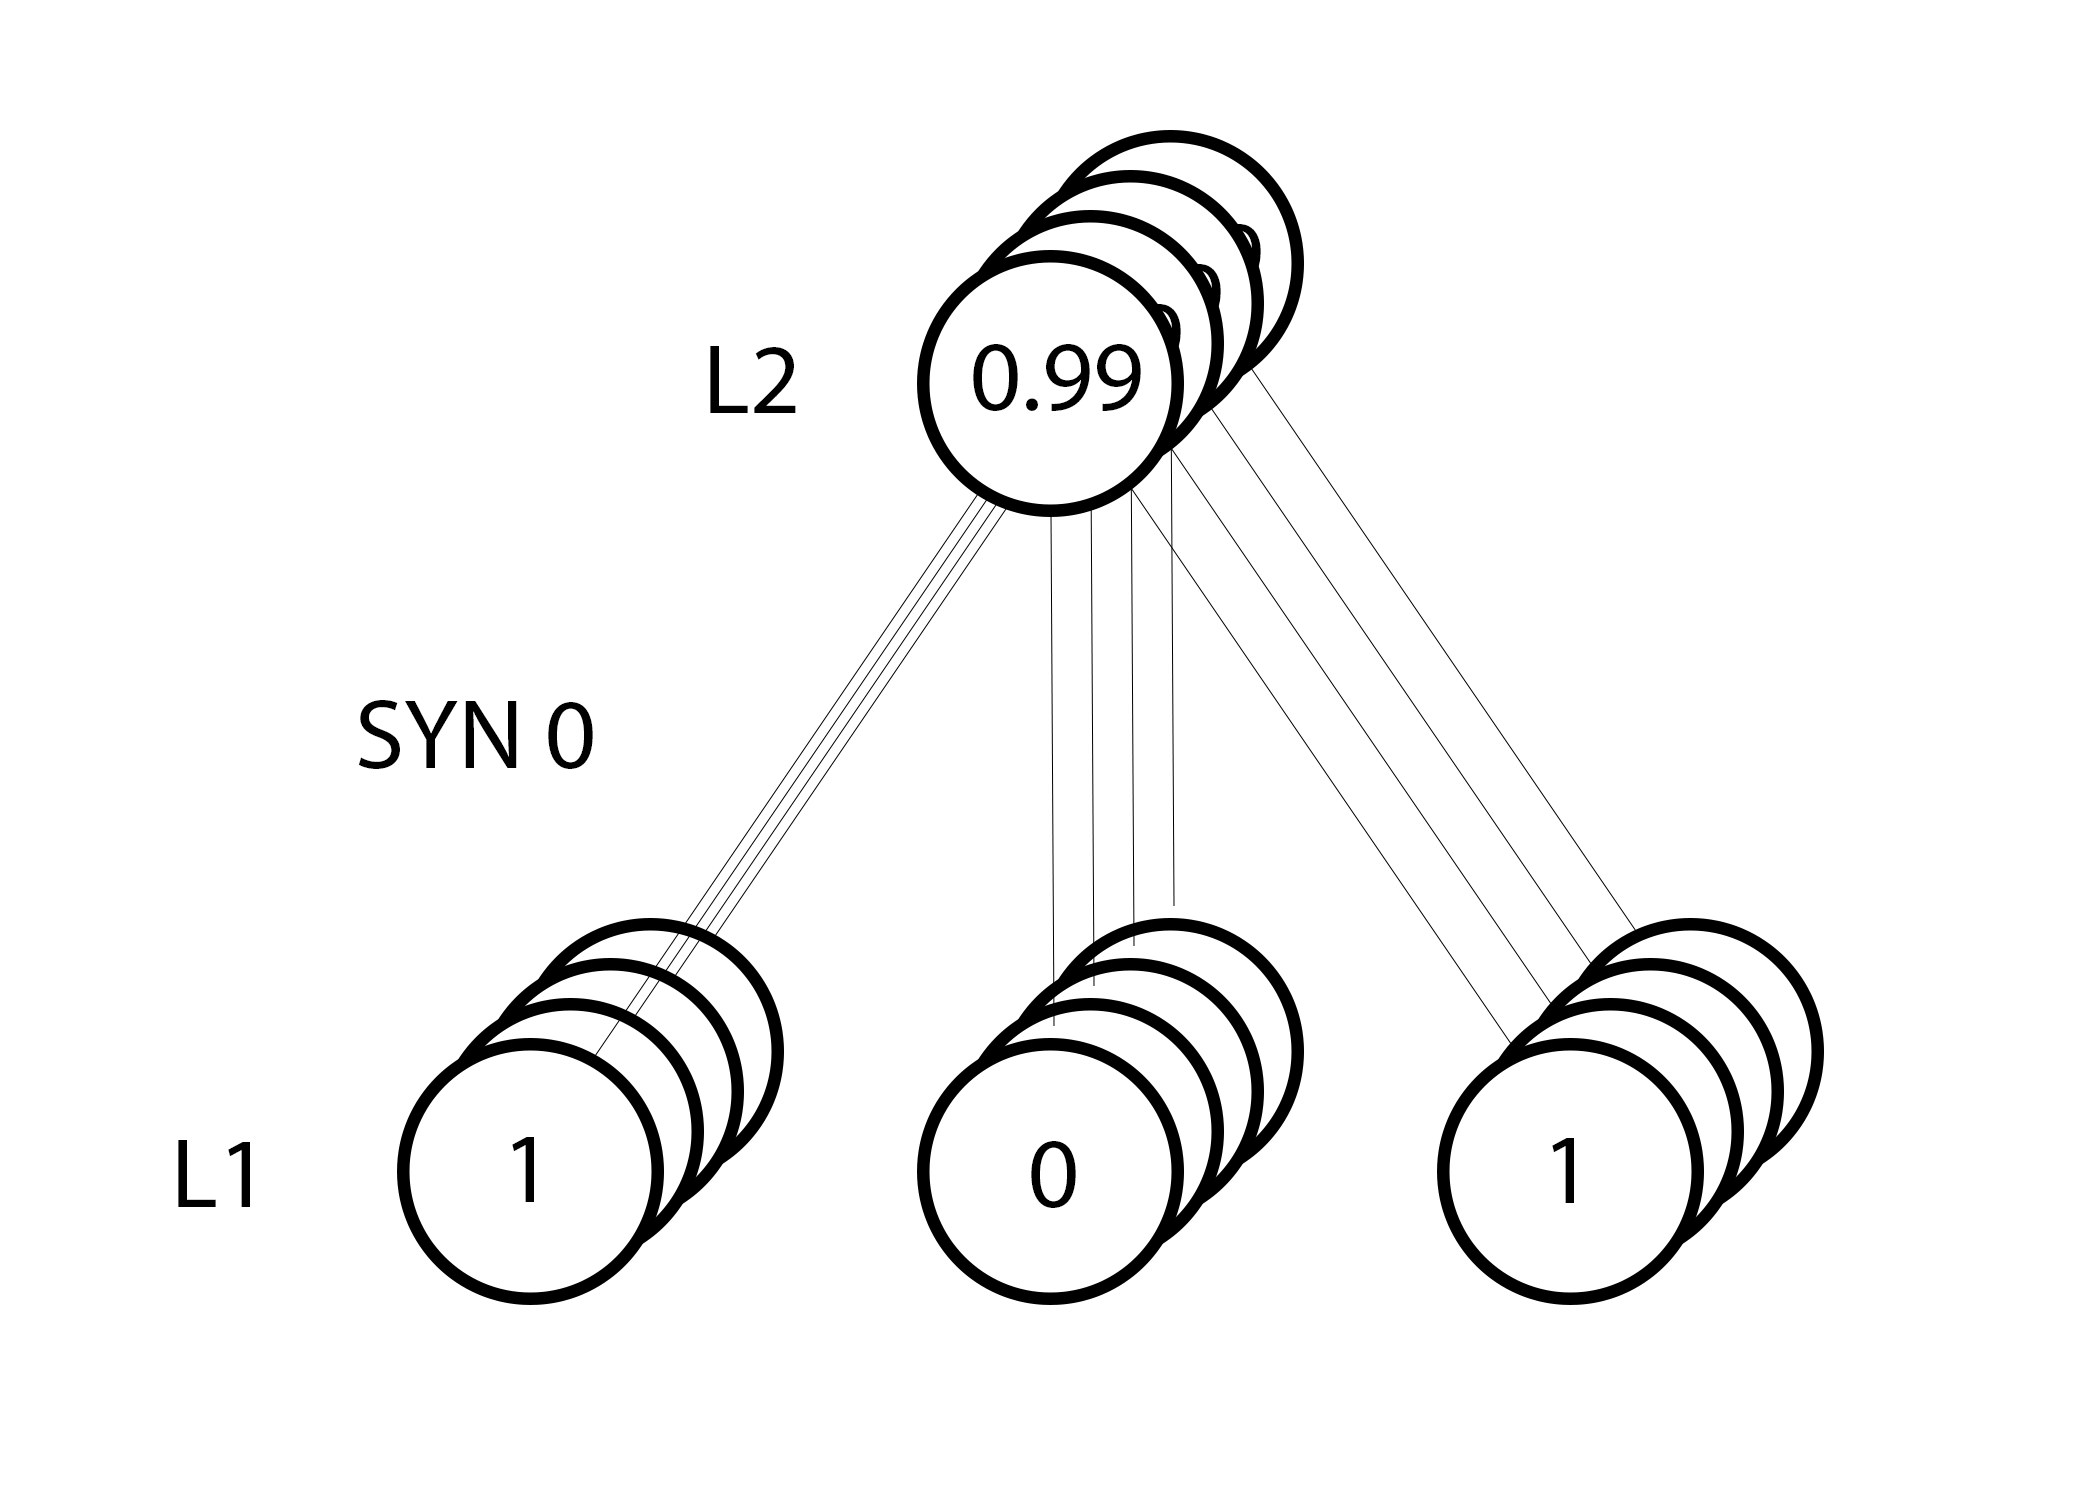
\includegraphics[width=0.6\linewidth,keepaspectratio]{ttn14}
\end{center}
However, because we're using a "full batch" configuration, we're doing the above step on all four training examples. 
\end{frame}

%%%%%%%%%%%%%%%%%%%%%%%%%%%%%%%%%%%%%%%%%%%%%%%%%%%
\begin{frame}[fragile] \frametitle{Explanation}
Let's update the far left weight (9.5): weight\_update = input\_value * l1\_delta
\begin{itemize}
\item It computes the weight updates for each weight for each training example, sums them, and updates the weights, all in a simple line. 
\item Play around with the matrix multiplication and you'll see it do this! 
\end{itemize}
\end{frame}

%%%%%%%%%%%%%%%%%%%%%%%%%%%%%%%%%%%%%%%%%%%%%%%%%%%
\begin{frame}[fragile] \frametitle{Output}
\begin{lstlisting}
Output After Training:
[[ 0.00966449]
 [ 0.00786506]
 [ 0.99358898]
 [ 0.99211957]]
\end{lstlisting}

Here are some good places to look in the code: 
\begin{itemize}
\item Compare l1 after the first iteration and after the last iteration.
\item Check out the ``nonlin'' function. This is what gives us a probability as output.
\item Check out how l1\_error changes as you iterate.
\item Take apart nonlin() line. Most of the secret sauce is here.
\item Check out dot(). Everything in the network prepares for this operation. 
\end{itemize}
\end{frame}


